%%%%%%%%%%%%%%%%%%%%% chapter.tex %%%%%%%%%%%%%%%%%%%%%%%%%%%%%%%%%
%
% sample chapter
%
% Use this file as a template for your own input.
%
%%%%%%%%%%%%%%%%%%%%%%%% Springer-Verlag %%%%%%%%%%%%%%%%%%%%%%%%%%


\chapstarthook{El contenido del cap�tulo corresponde con el art�culo: \textbf{J.A. Aguilar, I. Garrig{\'o}s, J.-N. Maz{\'o}n, J. Trujillo. Web Engineering Approaches for Requirements Analysis - A Systematic Literature Review. 6th Web Information Systems and Technologies (WEBIST 2010), Vol. 2, pp. 187-190, 2010.}}

\chapter{Web Engineering Approaches for Requirements Analysis - A Systematic Literature Review}
\label{c3} % Always give a unique label
% use \chaptermark{}
% to alter or adjust the chapter heading in the running head


%This chapter describes a standard and integrated model-driven
%framework with which to design each component of a data warehouse.
%Once this framework is defined, the focus is on the multidimensional
%modeling of the data warehouse repository. This chapter specifically
%defines a conceptual multidimensional model and how it is translated
%to a relational-based logical representation by using a model-driven
%approach. The advantages of using the model-driven development to
%design data warehouses are also enumerated. The content of this
%chapter corresponds with the part of the approach shaded in the
%figure below.

\begin{figure}[h!]
  \begin{center}
    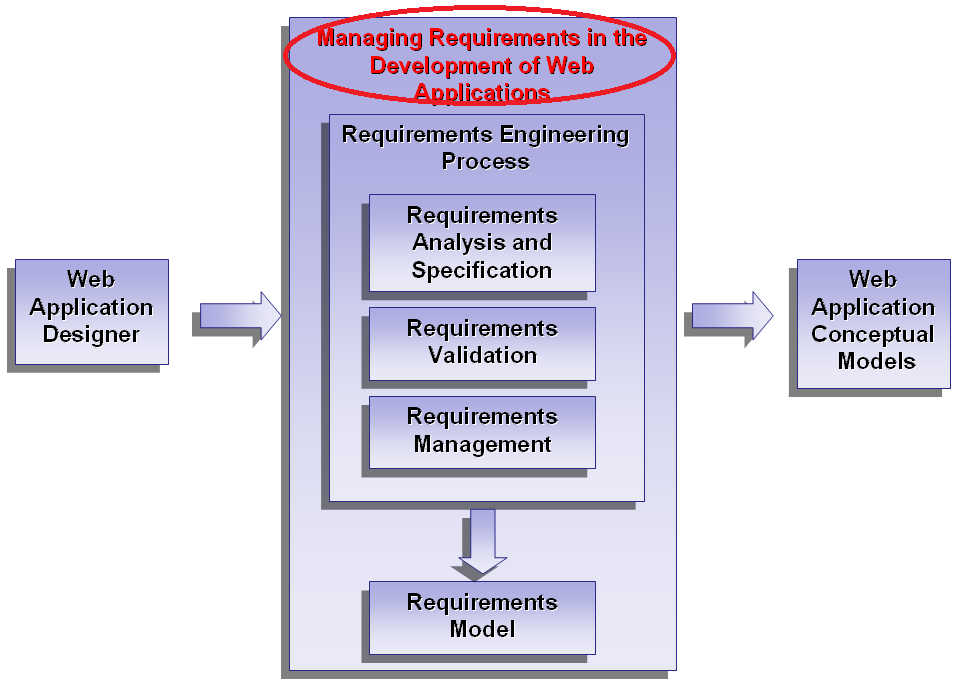
\includegraphics[width=0.7\textwidth]{img/PropuestaCapSLR.png}
  \end{center}
  %\caption{} \label{}
\end{figure}

El cap�tulo presenta una revisi�n sistem�tica de la literatura con el fin de obtener el estado de la cuesti�n en lo referente a m�todos para la especificaci�n, an�lisis y modelado de requisitos en ingenier�a Web as� como las herramientas de soporte ofrecidas por cada uno de los m�todos considerados. Los resultados obtenidos muestran, entre otras cosas, que gran parte de las metodolog�as Web no ofrecen un soporte integral en la etapa de an�lisis y especificaci�n de requisitos.
%The content of this chapter is a paper published in \emph{Decision
%Support Systems}. This journal focuses on contributions to the
%concepts and operational basis for decision support systems and
%techniques for implementing and evaluating decision support systems.
%This journal specifically encourages the following topics:
%artificial intelligence, data base management, decision theory,
%economics, linguistics, management science, mathematical modeling,
%amongst others. The common thread of articles published in the
%journal is their relevance to theoretical and technical issues for
%decision support systems. As data warehousing has been widely
%accepted as a key technology through which organizations can improve
%their abilities in data analysis and decision support, this journal
%is an important forum of publication for research in the data
%warehouse domain. Finally, it should be mentioned that this journal
%had an \emph{impact factor} of \emph{1.119} in 2007, according to
%the \emph{Thomson's Science Citation Index (SCI)}
%(\url{http://www.isiwebofknowledge.com/}).


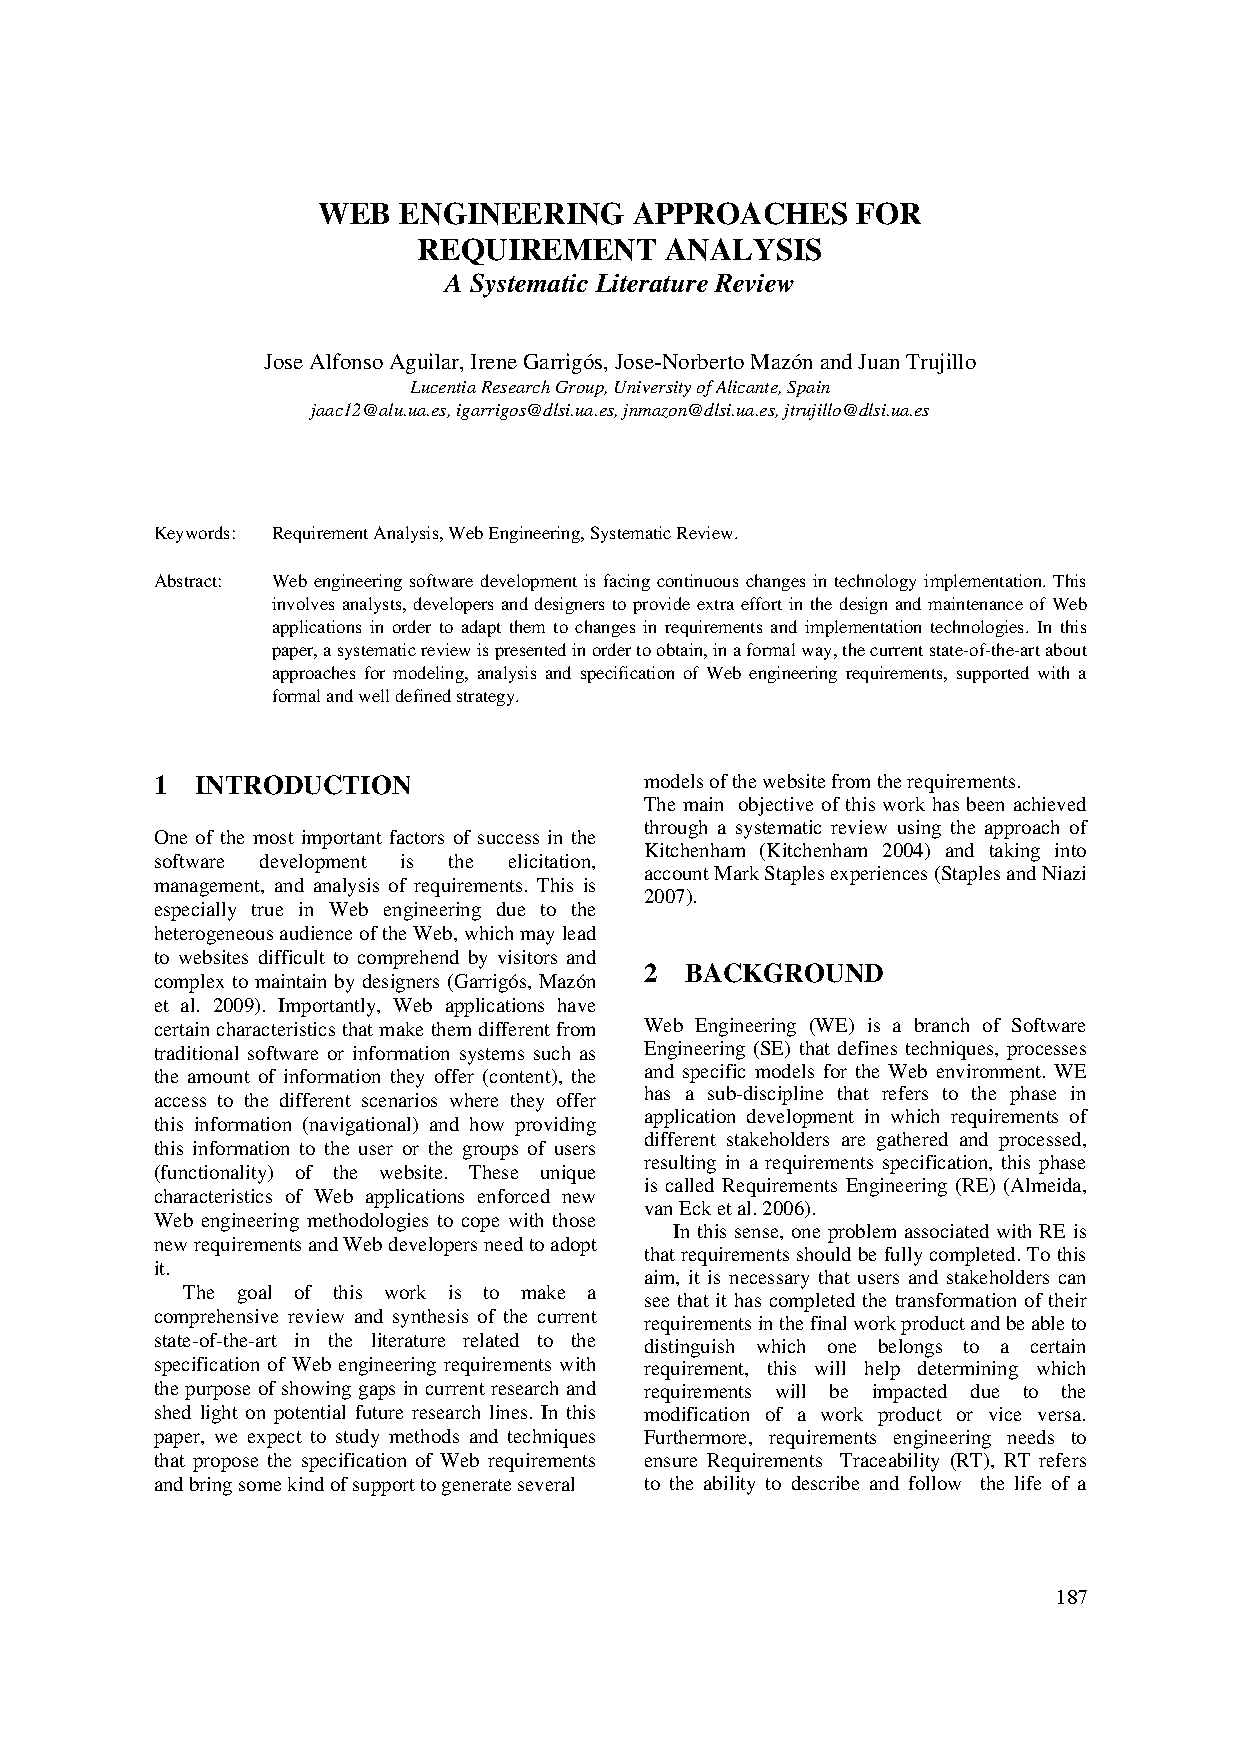
\includepdf[openright=true,pages={1-4}]{papers/WEBIST2010.pdf}



%
